\documentclass{yagoexam}
\usepackage{multicol}
\usepackage{color}
\usepackage{amsmath, amssymb, amsfonts, cancel, xfrac, siunitx, bm}
\usepackage{pifont}
\usepackage{braket}
\usepackage{gensymb}
\usepackage{graphicx, float, longtable, booktabs, mathrsfs}
\usepackage{mathrsfs}
%\usepackage[american, siunitx]{circuitikz}
\usetikzlibrary{positioning, calc}

%%%%%%%%%%%%%%%% INFO %%%%%%%%%%%%%%%%% 
\class{Controle Digital} % disciplina
\examname{Prova 3} % prova
\schoolyear{2019.2} % ano letivo
\examdate{11/02/2020} % data da prova
\teacher{Yago Pessanha} % você
%%%%%%%%%%%%%%%%%%%%%%%%%%%%%%%%%%%%%%%

\begin{document} 
	
%%%%%%%%%%%%%%%% LOGOS %%%%%%%%%%%%%%%% 
\makelogos{_rfb.png} % primeira img
{Macaé} % campus
{_iff.png} % segunda img
%%%%%%%%%%%%%%%%%%%%%%%%%%%%%%%%%%%%%%%%
	
%%%%%%%%%%%%%%%% TABELA %%%%%%%%%%%%%%%% 
\maketitle
%%%%%%%%%%%%%%%%%%%%%%%%%%%%%%%%%%%%%%%%

%%%%%%%%%%%%%% INSTRUÇÕES %%%%%%%%%%%%%%
\begin{itemize}
		
	\item Esta avaliação contém \numquestions\ questões e \numpages\ páginas. Confira se todas as páginas estão presentes.
	
	\item A avaliação tem duração de 150 minutos.
		
	\item Calculadoras poderão ser usadas. 
	
	\item Na última página desta prova encontra-se o apêndice com a tabela de Transformadas $\mathcal{Z}$.
		
	\item É proibido portar livros, manuais e anotações.
		
	\item Assine o seu nome à caneta no espaço apropriado, além de preencher a sua turma.
		
	\item A avaliação deverá ser feita à lápis, exceto as questões de múltipla escolha (quando existirem).  
		
	\item Por favor, desenhe um \framebox{retângulo} ao redor de sua resposta, sempre que possível. 
		
	\item A interpretação das questões faz parte da avaliação.
		
	\item Responda cada questão em sua área destinada para resposta.
	
	%\item Questões de múltipla escolha só serão consideradas com os devidos cálculos (quando exigirem).
		
	\item Respostas incompletas ou faltando todos os passos necessários receberão uma nota parcial.
		
\end{itemize}
\newpage % End of cover page
%%%%%%%%%%%%%%%%%%%%%%%%%%%%%%%%%%%%%%%%
	
%%%%%%%%%%%%%%%% QUESTÕES %%%%%%%%%%%%% 
\begin{questions}
	
	\question[15]
	Considere um sistema discreto, causal, linear e invariante no tempo com a seguinte \textbf{função de transferência}:
	
	$$H(z) = \dfrac{1}{1+a_1z^{-1}}$$
	
	Se a saída do sistema é a sequência $y[n]$
	quando a entrada é a sequência $u[n]$, qual é o valor de \bm{$a_1$}? \textit{Dica:} transforme a função de transferência em equação de diferenças.
	
	  \begin{figure}[h]
	\caption{\label{q1}Sequências $u[n]$ e $y[n]$ para a questão 1}
	\begin{center}
		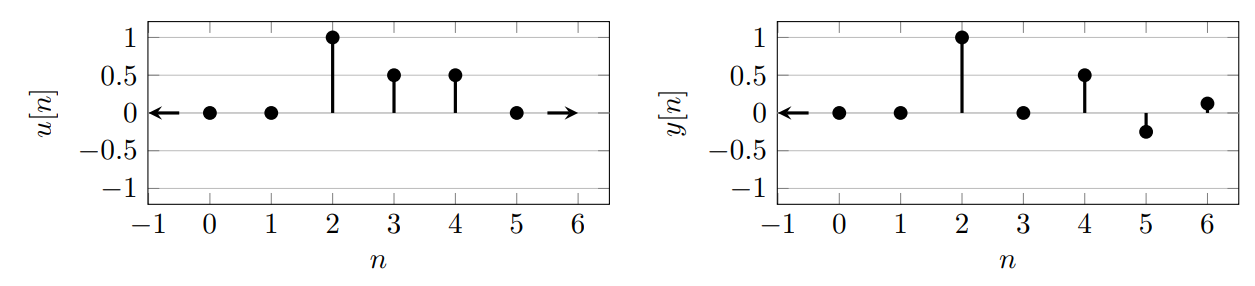
\includegraphics[scale=1]{q1.PNG}
	\end{center}
    \end{figure} 
    
    \newpage
    
    \question[10]
    Considere o seguinte diagrama de blocos em \textbf{série} de sistemas discretos, causais, lineares e invariantes no tempo:
    
	  \begin{figure}[h]
	\caption{\label{q2}Diagrama de blocos em série para a questão 2}
	\begin{center}
		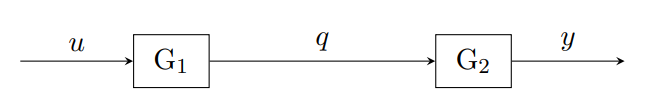
\includegraphics[scale=1]{q2.PNG}
	\end{center}
    \end{figure}
    
    onde
    
    $$q[n] = 0.5q[n - 1] + 2u[n]$$
    $$y[n] = -0.75y[n - 1] + q[n]$$
    
    \vspace{0.5cm}
    
    \begin{parts}
    
    \part Qual é a \textbf{função de transferência} do sistema em \textbf{série}, isto é, qual é a função de transferência que relaciona a entrada $u$ e a saída $y$?
    
    \vspace{8cm}
    
    \part O sistema em \textbf{série} é \textbf{estável}?

    \end{parts}
    
    \newpage
    
    \question[15]
    Considere um sistema causal, linear e invariante no tempo cuja \textbf{resposta ao impulso} $h$ é:
	
	$$h[n] = \alpha^ns[n] \qquad \forall n,$$
	
	onde $s[n]$ é a sequência do \textbf{degrau unitário}. Sob qual \textbf{condição} o sistema é \textbf{estável}?

    \newpage
    
    \question[15]
    Considere a função de transferência \textbf{contínua} de um filtro \textit{Butterworth} de primeira ordem com frequência de corte igual a 1 rad/s.
    
    $$H(s) = \dfrac{1}{s+1}$$
    
    \vspace{0.5cm}
    
    \begin{parts}
    
    \part \textbf{Discretize} este filtro usando a transformação bilinear \textbf{sem} \textit{prewarping}. Adote $T = 1$ s.
    
    \vspace{6cm}
    
    \part Desenhe o \textbf{diagrama polo-zero} de $H(z)$.
    
    \vspace{7cm}
    
    \part Este filtro é \textbf{estável}?
    
    \end{parts}
    
    \newpage
    
    \question[15]
    Considere um sistema em \textbf{malha fechada} cuja \textbf{equação característica} seja:
    
    $$D(z) = z^2 - z + 2 = 0$$
    
    \vspace{0.5cm}
    
    \begin{parts}
    
    \part Utilizando o \textbf{critério de Jury}, mostre que este sistema é \textbf{instável}.
    
    \vspace{6cm}
    
    \part Utilizando o \textbf{critério de Routh Hurwitz modificado} e a transformação bilinear do plano $\mathcal{W}$, mostre que este sistema é \textbf{instável}.
    
    \vspace{6cm}
    
    \part Utilizando o \textbf{critério da localização dos polos} da equação característica, mostre que este sistema é \textbf{instável}.
    
    \end{parts}
    
    \newpage
    
    \question[30]
    Considere o \textbf{diagrama de blocos} de um sistema em malha fechada representado pela figura \ref{q6}. 

	  \begin{figure}[h]
	\caption{\label{q6}Diagrama de blocos para a questão 6}
	\begin{center}
		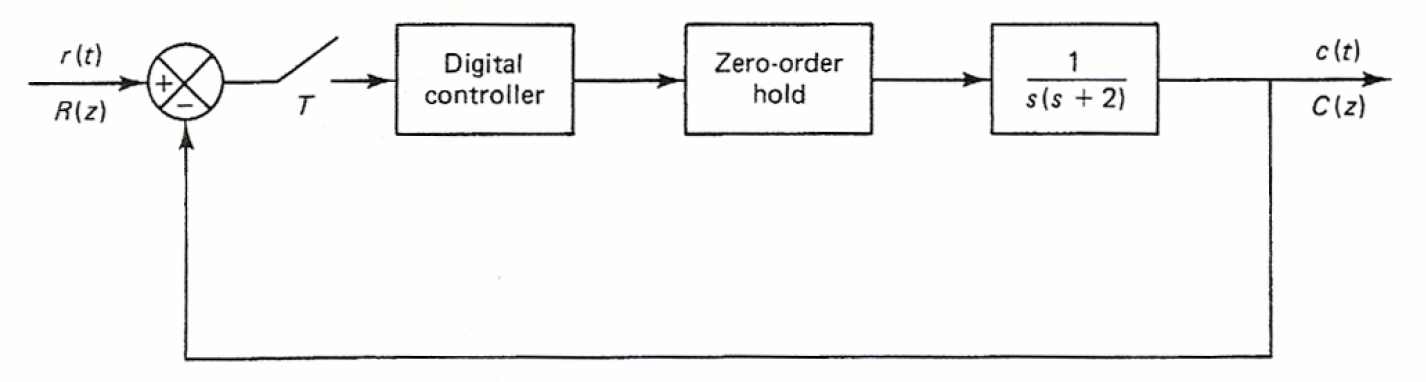
\includegraphics[scale=0.8]{q6.PNG}
	\end{center}
    \end{figure}    
    
    Projete um \textbf{controlador digital}, por \textbf{emulação}, utilizando a técnica do \textbf{lugar das raízes}, sabendo que é desejado que os polos dominantes tenham um \textbf{fator de amortecimento} de $0,5$ e um \textbf{tempo de acomodação} de $2$ s. Assuma T = $T_d/9$ s. Determine ainda o \textbf{erro em regime permanente} para uma entrada $r(t) = e^2  t$, para todo $t \geq 0$, onde $e$ é uma constante matemática, conhecida como o número de Euler.
    
    
    \newpage
    
    \mbox{}

    \newpage
    
    \mbox{}

    \newpage
    
\end{questions}
    
        \begin{minipage}{2in}
{\fontfamily{qcr}\selectfont
{\LARGE \textbf{APÊNDICE}} 
}
\end{minipage}
\hfill
\begin{minipage}{1.3in}
{\fontfamily{qcr}\selectfont
{\LARGE \textbf{}} 
}
\end{minipage}
\\ \rule[0.5ex]{\textwidth}{1.2pt}
\vspace{0.1cm}


\begin{table}[!ht]
	\caption{Transformada $Z$}\label{ztable}
	\vspace{0.5cm}
\setlength{\arrayrulewidth}{0.5mm}
\setlength{\tabcolsep}{20pt}
\renewcommand{\arraystretch}{1.5}

\begin{tabular}{ |p{7cm}|p{7cm}|  }
\hline
\textbf{Funções} & \textbf{Transformada $Z$} \\
\hline
$\delta _{t,nT}$  & $\displaystyle z^{-n}(n\geq 0)\vspace{0.16in}$  \\
$x[n]$  & $\displaystyle\frac{z}{z-1}\vspace{0.16in}$    \\
$t$  & $\displaystyle \frac{Tz}{(z-1)^2}\vspace{0.16in}$    \\
$t^2$  & $\displaystyle \frac{T^2z(z+1)}{(z-1)^3}\vspace{0.16in}$    \\
$e^{-at}$ & $\displaystyle\frac{z}{z-e^{-aT}}\vspace{0.16in}$    \\
$te^{-at}$    & $\displaystyle\frac{Tze^{-aT}}{(z-e^{-aT})^{2}}\vspace{0.16in}$  \\
$t^{2}e^{-at}$ & $\displaystyle\frac{T^{2}ze^{-aT}(z+e^{-aT})}{%
(z-e^{-aT})^{3}}\vspace{0.16in}$  \\
$\sinh at$ & $\displaystyle\frac{z\sinh aT}{z^{2}-2z\cosh aT+1}\vspace{0.16in%
}$    \\
$\cosh at$ & $\displaystyle\frac{z(z-\cosh aT)}{z^{2}-2z\cosh aT+1}\vspace{%
0.16in}$  \\
\hline
\end{tabular}
\end{table}
    
	


%%%%%%%%%%%%%%%%%%%%%%%%%%%%%%%%%%%%%%%%

\end{document}
